\section{实验}
\label{sec:experiments}
\subsection{实验协议、基线与统计单位}
\paragraph{构造基准。}
资源参与模拟器包含 128 个智能体、8 个时间步和 3 个轨迹通道。机制库有 200 个候选，由 10 个注意参数、10 个参与参数与 2 个退出参数组合而成，每个候选使用 8 个种子。4 个历史活动和 4 个可访问规则探针支持校准与取证，开发、测试各含 3 个相互影响的活动。历史中分别出现候补和转发，冲突仅在探针和后续划分中启用，因此不是每个规则组件都有经验训练覆盖。真实参数为 $(0.90,0.30,0.27)$，其中退出参数不恰好落在候选的两级网格上。历史核查包含 96 条意图记录，缺失概率为 20\%；取证池有 160 条记录，缺失概率为 15\%，均按 MCAR 生成。每条记录成本为 1。候选推演共享随机数，真值采用独立种子。内部名称 \texttt{SocioVerse\_Campus} 指这个构造基准，不是 SocioVerse 官方数据。

\paragraph{冻结选择与评测。}
自动化研究控制器对唯一算法文件提出并评测了 60 个不同候选，保留 10 个、回退 50 个，所有假设和源码版本均归档。固定评测器、预算网格 $\{0,2,4,8,12,16\}$ 与缓存不参与该循环的优化。最优方法在第一次报告测试结果前冻结，后续重跑用于核验复现，并非新的保留集。原指标是合并轨迹 RMSE 的归一化梯形积分：
\begin{equation}
 A_{\mathrm{pool}}=\frac1{16}\sum_{j=1}^{J}
 (b_j-b_{j-1})\frac{R_{\mathrm{pool}}(b_j)+R_{\mathrm{pool}}(b_{j-1})}{2}.
 \label{eq:auc}
\end{equation}
轨迹误差以人口比例计。原测试的三个活动共享人群、预算和冲突，不能把它们的时间格当作独立样本。

为量化变异，冻结后的补充协议生成了 24 个独立世界，改变人群与模拟随机过程，同时固定训练观测、取证证据和三个活动模板。对每个模板，把式~\eqref{eq:auc} 中的合并 RMSE 换成活动内 RMSE 得到 $A_e$，再定义 $A_{\mathrm{macro}}=\frac13\sum_eA_e$。以整个世界为单位做 bootstrap 重采样，共 2,000 次、固定随机种子，保留同一世界内活动的依赖。随机查询的多次重复先在世界内平均。各表报告每个模板的 24 次独立实现及条件 95\% 区间；这不是 72 个互不相关的活动，也不覆盖新训练集或新领域。补充协议是在原测试被查看后才确定的，因此属于冻结后的扩展，而非事先保留、完全未触碰的第二基准。

\paragraph{对比策略。}
Random 均匀随机选择可获取记录；Entropy 最大化单位成本的二元预测熵；ParamIG 使用 $h(q_r)-\sum_mw_mh(p_{mr})$，其中 $h$ 为二元熵；Standard OED 以历史轨迹而非组合探针的预测方差缩减为目标，它只代表这一特定目标选择，并不涵盖所有目标导向设计。原对照从均匀相容权重开始，完整方法（Full）从式~\eqref{eq:weights} 开始。因此，我们增加同先验版本，以单独判断取证作用。被动基线包括历史均值统计模型、未校准混合模型、仅过程校准、仅轨迹校准和 V1 被动联合校准。这些是合成统计基线，不替代尚未执行的原产品或 LLM 基线。

\subsection{RQ1：相容集合是否保留了有用的机制不确定性？}
最终硬集合包含 170 个候选，但只有 12 个拥有非零 float32 权重，超过 $10^{-4}$ 的只有两个。初始有效机制数 $(\sum_mw_m^2)^{-1}$ 为 \ESS，最大权重为 \MaxWeight。最重机制约为 $(0.4167,0.6833,0.42)$，与生成系统的注意、参与参数明显不同。因此，较小的轨迹误差不能证明机制恢复成功。

额外的歧义诊断只利用历史与探针选择候选对，不读取测试结果。所选候选对的历史轨迹 RMSE 为 \HistoryPair，探针 RMSE 为 \ProbePair。两者参数不同，但这组实测候选并没有证明组合下分歧发生剧烈放大。机制歧义仍然是合理的研究问题，只是这一诊断不足以证明基准实现了最强形式的歧义放大。

原单点基线与 Full 使用不同的选点损失；匹配 MAP 对照则把全部质量放在进化校准下权重最大的候选上。表~\ref{tab:macro} 中，Full 的宏平均 AUC 为 \MacroFull，匹配 MAP 为 \MacroMAP，在人口比例尺度上差别极小。表~\ref{tab:paired} 给出逐活动配对差值，而不是通过两个边际区间是否重叠来推断显著性。当前结果没有建立保留混合分布能实质提升准确性的证据。
\begin{table}[tbp]
\centering
\caption{宏平均 AUC $\times10^3$ 及其相对 Full 的描述性均值差。区间是均值的世界 bootstrap 区间，不是预测区间。}
\label{tab:macro}
\scriptsize
\setlength{\tabcolsep}{3pt}
\begin{tabular}{lrr}
\toprule
方法 & 宏平均 AUC & 相对 Full 的差值 \\
\midrule
Full & 7.0635 [6.0247, 8.0995] & +0.0000 \\
匹配 MAP & 7.0655 [6.0267, 8.1012] & +0.0019 \\
同先验 Random & 7.0589 [6.0192, 8.0962] & -0.0046 \\
移除组合目标 & 7.0635 [6.0247, 8.0995] & +0.0000 \\
移除批量条件化 & 7.0635 [6.0247, 8.0995] & +0.0000 \\
取消参数共享* & 39.8238 [38.5402, 41.0323] & +32.7602 \\
\bottomrule
\end{tabular}
\end{table}


\paragraph{未知规则诊断。}
我们分别引入候选未建模的候补退出、两跳同伴传播、两者组合，以及较强的交通取消冲击，候选规则始终冻结。区间诊断在观察到活动结果后触发：如果超过 20\% 的时间通道格落在逐点 90\% 预测区间外，则告警。表~\ref{tab:stress} 和图~\ref{fig:stress} 区分误报率与检出率。不同活动的误报率差异较大，对候补、传播偏移的检出也较弱；强交通冲击则在每个模板的全部 24 个世界中被检出。此时 bootstrap 区间可能退化为端点；样本检出率为 1，不代表总体灵敏度完美。
\begin{table}[tbp]
\centering
\caption{Full 的事后区间告警率（百分比）与 95\% 世界 bootstrap 区间。“无偏移”衡量误报率；24 个世界中端点比例的区间可能退化。}
\label{tab:stress}
\scriptsize
\setlength{\tabcolsep}{3pt}
\begin{tabular}{lrrr}
\toprule
真值规则 & 活动 1 & 活动 2 & 活动 3 \\
\midrule
无偏移 & 4.2 [0.0, 12.5] & 25.0 [8.3, 41.7] & 8.3 [0.0, 20.8] \\
候补偏移 & 12.5 [0.0, 25.0] & 20.8 [4.2, 37.5] & 8.3 [0.0, 20.8] \\
传播偏移 & 8.3 [0.0, 20.8] & 16.7 [4.2, 33.3] & 16.7 [4.2, 33.3] \\
两者叠加 & 12.5 [0.0, 25.0] & 12.5 [0.0, 25.0] & 16.7 [4.2, 33.3] \\
交通冲击 & 100.0 [100.0, 100.0] & 100.0 [100.0, 100.0] & 100.0 [100.0, 100.0] \\
\bottomrule
\end{tabular}
\end{table}

\begin{figure}[tbp]
\centering
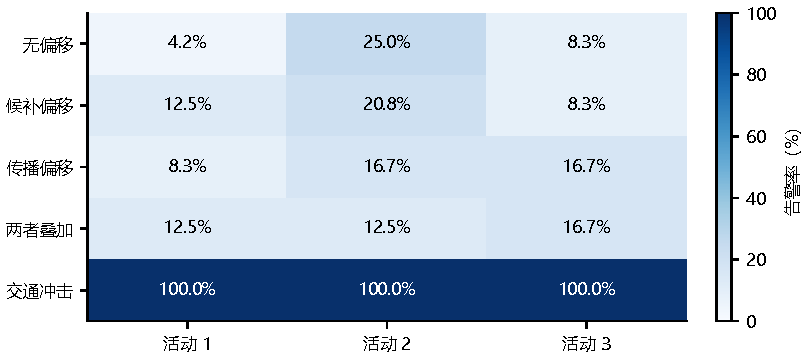
\includegraphics[width=.83\linewidth]{stress_alarms.pdf}
\caption{合成世界中 Full 的事后告警率。“无偏移”是误报对照。对强取消冲击的较好检出，与对候补、传播偏移的较弱检出同时存在。区间见表~\ref{tab:stress}。}
\label{fig:stress}
\end{figure}
原评测器要求认识方差较低且 RMSE 超过 $0.08$ 才告警，该诊断在补充实验的候补与传播扰动中从未触发。表~\ref{tab:stress_magnitude} 同时报告真值位移：部分模板的候补扰动很小，因此不能把不同偏移的漏检都解释为同等严重的失败。两种诊断均依赖已经实现的结果，不是事前预警。失配候选之间的一致意见，本身无法识别遗漏规则。

\subsection{RQ2：什么改善了证据效率，又是什么得到了加速？}
原开发 AUC 从 \InitialDev\ 降至 \FinalDev，在同一开发集自适应选择后下降 \DevReduction\%。冻结测试 AUC 为 \TestAUC。这是所选预测器在固定合成评测上的证据，不是相对外部最优方法的提升百分比。独立世界的宏平均结果是不同统计量，不能替换合并测试分数。

表~\ref{tab:acquisition_original} 与图~\ref{fig:curves} 上排给出原始比较。Full 的较低曲线包含进化校准的收益，其他取证器则从均匀相容权重出发。表~\ref{tab:acquisition_matched} 改为同先验比较后，表面的取证优势消失。同先验 Random 的宏平均 AUC 为 \MacroRandom，略低于 Full 的 \MacroFull。差异很小，近乎平坦的曲线说明初始集中的权重在很大程度上已决定预测。这些控制避免了把校准收益归到查询准则上。
\begin{table}[tbp]
\centering
\caption{原始对照：校准与取证策略同时变化。逐活动 AUC $\times10^3$，括号为 95\% 世界 bootstrap 区间；24 个独立世界，固定训练数据、证据与模板。}
\label{tab:acquisition_original}
\scriptsize
\setlength{\tabcolsep}{3pt}
\begin{tabular}{lrrr}
\toprule
方法 & 活动 1 & 活动 2 & 活动 3 \\
\midrule
Random & 17.82 [17.23, 18.39] & 19.03 [18.10, 20.01] & 14.96 [14.46, 15.44] \\
Entropy & 12.94 [12.27, 13.64] & 10.15 [9.21, 11.16] & 8.19 [7.32, 9.14] \\
ParamIG & 12.98 [12.34, 13.68] & 10.80 [10.06, 11.59] & 8.56 [7.50, 9.73] \\
Standard OED & 23.59 [22.32, 24.75] & 27.44 [24.79, 30.05] & 21.58 [19.34, 23.61] \\
Full & 4.19 [3.38, 5.07] & 10.85 [8.78, 12.85] & 6.15 [3.98, 8.65] \\
\bottomrule
\end{tabular}
\end{table}

\begin{table}[tbp]
\centering
\caption{同先验取证对照：所有方法采用进化先验。逐活动 AUC $\times10^3$，括号为 95\% 世界 bootstrap 区间；24 个独立世界，固定训练数据、证据与模板。}
\label{tab:acquisition_matched}
\scriptsize
\setlength{\tabcolsep}{3pt}
\begin{tabular}{lrrr}
\toprule
方法 & 活动 1 & 活动 2 & 活动 3 \\
\midrule
同先验 Random & 4.19 [3.38, 5.07] & 10.84 [8.77, 12.84] & 6.15 [3.98, 8.65] \\
同先验 Entropy & 4.19 [3.38, 5.07] & 10.85 [8.78, 12.85] & 6.15 [3.98, 8.65] \\
同先验 ParamIG & 4.19 [3.38, 5.07] & 10.85 [8.78, 12.85] & 6.15 [3.98, 8.65] \\
同先验 Standard OED & 4.19 [3.38, 5.07] & 10.85 [8.78, 12.85] & 6.15 [3.98, 8.65] \\
Full & 4.19 [3.38, 5.07] & 10.85 [8.78, 12.85] & 6.15 [3.98, 8.65] \\
\bottomrule
\end{tabular}
\end{table}

\begin{figure}[tbp]
\centering
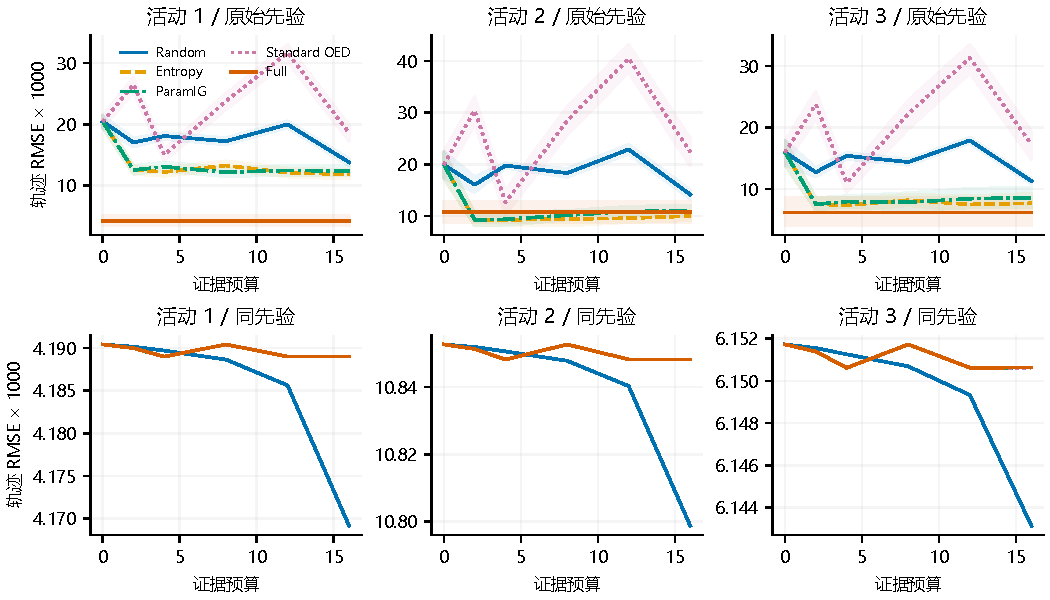
\includegraphics[width=\linewidth]{budget_curves.pdf}
\caption{逐活动展示的合成预算—轨迹误差曲线。上排为原校准策略，阴影是条件 95\% 世界 bootstrap 区间；下排全部使用进化先验，曲线几乎重合。下排保持绝对数值，但各图尺度不同，不能把其微小起伏与上排效应量直接作视觉比较。}
\label{fig:curves}
\end{figure}

\paragraph{评分微基准。}
使用相同候选、缓存预测、概率和成本，比较协方差评分与显式枚举二元结果。10 组 GPU 同步配对计时交替执行顺序。表~\ref{tab:timing} 报告冻结权重下 \FrozenSpeed\ 倍、均匀相容权重下 \UniformSpeed\ 倍的配对加速比中位数，以及最大评分残差。图~\ref{fig:evolution} 展示原始计时。参考实现是所提供的循环枚举版本；充分向量化的枚举器可以共享相当一部分计算。因此，这些测量证明的是局部实现优势，不是相对所有优化 OED 的普遍加速，也不是渐近复杂度改进。
\begin{table}[tbp]
\centering
\caption{10 次同步 GPU 配对计时，执行顺序交替。分别计算每一对的加速比再取中位数，因此不必等于两类时间中位数之比。}
\label{tab:timing}
\scriptsize
\setlength{\tabcolsep}{3pt}
\begin{tabular}{lrrrr}
\toprule
先验 & 协方差（毫秒） & 枚举（毫秒） & 配对加速比中位数 & 最大残差 \\
\midrule
冻结先验 & 0.773 & 178.17 & 217.95 & 9.08e-16 \\
均匀相容先验 & 0.747 & 191.85 & 275.16 & 1.38e-10 \\
\bottomrule
\end{tabular}
\end{table}

指定的冻结全量评测在 RTX 4060 Laptop GPU 上用时 \TestRuntime\ 秒，报告 PyTorch 峰值分配显存 \TestVRAM\ MB。它们仅对应缓存评测，不包含离线缓存生成和显卡驱动占用。开发试验约需 4 至 9 秒。小型缓存评测适合 8 GB 显存，但这不证明更大人群或更丰富机制库也能维持相同速度。

\subsection{RQ3：哪些改动经受住了受控消融？}
表~\ref{tab:ablations} 比较完整方法、四种移除设置以及匹配单点估计。移除组合目标或批量条件化，汇总结果不变。这与权重近乎单点的现象一致：若似然无法移动足够多的质量，改变查询选择也很难影响预测。取消共享会使结果变差，但该库使用逐活动独立参数排列，同时改变先验和假设空间。因此，这一结果描述的是相应实现，不是参数共享收益的纯因果估计。
\begin{table}[tbp]
\centering
\caption{冻结方法消融。星号表示同时改变了先验或单点选择目标。逐活动 AUC $\times10^3$，括号为 95\% 世界 bootstrap 区间；24 个独立世界，固定训练数据、证据与模板。}
\label{tab:ablations}
\scriptsize
\setlength{\tabcolsep}{3pt}
\begin{tabular}{lrrr}
\toprule
方法 & 活动 1 & 活动 2 & 活动 3 \\
\midrule
Full & 4.19 [3.38, 5.07] & 10.85 [8.78, 12.85] & 6.15 [3.98, 8.65] \\
取消参数共享* & 47.19 [45.23, 49.01] & 21.17 [18.72, 23.61] & 51.11 [48.60, 53.35] \\
移除组合目标 & 4.19 [3.38, 5.07] & 10.85 [8.78, 12.85] & 6.15 [3.98, 8.65] \\
原单点估计* & 5.42 [4.71, 6.08] & 7.54 [5.92, 9.35] & 7.37 [5.78, 8.95] \\
匹配 MAP & 4.19 [3.38, 5.07] & 10.85 [8.78, 12.85] & 6.15 [3.99, 8.65] \\
移除批量条件化 & 4.19 [3.38, 5.07] & 10.85 [8.78, 12.85] & 6.15 [3.98, 8.65] \\
\bottomrule
\end{tabular}
\end{table}


开发轨迹说明了集中如何形成。R1--R7 引入轨迹加权并逐步收窄核宽，R30 把历史平均误差换成最差活动误差。R38 再次收窄核宽，但接受的改善仅约 $10^{-7}$，不应作为性能跃升。R58 引入式~\eqref{eq:distance} 的噪声归一化，是后期最大的一次改善。由于每次接受的修改都会成为下一轮起点，这些顺序决策并不是彼此独立的消融。全部 60 个分数和决定见附录~\ref{app:trials}。

群体目标与过程预测也存在取舍：开发 Brier 从 \DevBrierStart\ 变差为 \DevBrierEnd，冻结测试 Brier 为 \TestBrier。冻结测试逐点覆盖率为 \TestCoverage\%，平均宽度为 \TestWidth。边际覆盖率较高，不等于机制得到识别，也不等于模型类外不确定性已校准。独立世界的不确定性表（表~\ref{tab:uncertainty}）分别报告认识与随机方差；在最终权重下，前者远小于后者。
\begin{figure}[tbp]
\centering
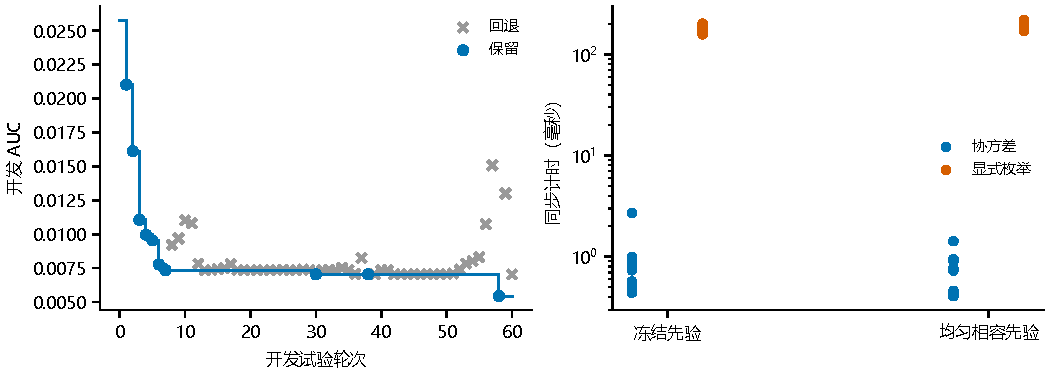
\includegraphics[width=\linewidth]{evolution_timing.pdf}
\caption{左：全部 60 个开发候选及保留分数轨迹，回退试验同样保留。右：每类先验的全部 10 组配对计时；对数坐标区分协方差与枚举成本，计时重复不作为独立活动样本。}
\label{fig:evolution}
\end{figure}

\subsection{第二阶段：非坍缩校准与同先验主动取证}
\label{sec:round2}
\paragraph{保留 V1，单独验证其失效原因。}
第~\ref{sec:method} 节及第 4.1--4.4 节报告原始 V1 研究。本节针对一个具体问题展开：如果校准后仍保留合理的候选机制，过程取证能否重新产生可测量的收益？我们保留 \texttt{eb641c2} 的代码、数据和原始结论，在独立分支预先固定新的压力场景、裁决护栏和 30 组开发配置。V1 与 V2 都在新场景上重新评测；不能把新旧基准的分数直接相减，再将差异全部归因于算法。

\paragraph{机制歧义的构造与统计单位。}
新配置采用 256 个智能体、8 个模拟种子、12 个时间步和 200 组候选机制。预先指定的两组机制为 $(a,b,d)=(.2,.95,.12)$ 与 $(.95,.2,.12)$，注意概率与参与概率的乘积相同。通过逆变换共同随机数耦合，二者生成相同的初始意图。历史活动分别启用候补或转发；组合活动同时启用候补通知触发的八邻居传播级联和强同时间冲突。这对机制的历史轨迹 RMSE 为 0.00000，组合探针及测试事件设计上的轨迹分歧为 0.28094。这是专门构造的交互压力测试，不是从真实行为数据拟合出的社会规律。

开发和测试分别使用 12 个与 24 个独立模拟世界。测试更换世界、过程审计和取证答案，事件设计仍与组合探针相同，因此它验证的是同一设计下的新世界复现，不是超出探针的新组合迁移。区间以整个世界为单位进行配对 bootstrap，保留世界内活动之间的依赖，逐活动另行报告。

\paragraph{校准公式与保留条件。}
在 V1 的历史相容支持集 $\mathcal C$ 上，设 $r_{etc}$ 为式~\eqref{eq:distance} 中的相对种子方差归一化项。V2 采用
\begin{align}
 E_m^{(2)}&=\frac{1}{2\sigma^2}\operatorname{mean}_{e,t,c}
 \frac{(\bar X_{metc}-H_{etc})^2}{r_{etc}}+\lambda\ell_m^{\mathrm{proc}},\\
 \ell_m^{\mathrm{proc}}&=-\frac{1}{|\mathcal O|}\sum_{j\in\mathcal O}
 [y_j\log p_{mj}+(1-y_j)\log(1-p_{mj})],\\
 w_{0m}^{(2)}&\propto\mathbf1[m\in\mathcal C]\exp(-E_m^{(2)}/T),\qquad
 T=\inf\{t\geq1:\,N_{\mathrm{eff}}(w_0(t))\geq8\}.
 \label{eq:v2-calibration}
\end{align}
实现中通过二分求解温度，并留出很小的数值余量。MCAR 缺失标签不贡献对数似然；意图记录中未观测的查看状态仍按 $p_{mj}=a_mb_m I_j$ 边缘化。支持集筛选条件不变。上述平均残差对应最终选中的 V2；搜索也包含最坏活动残差版本。Gibbs 温度可以解释为熵正则强度，但这里直接约束的有效机制数对应二阶 R\'enyi 熵，并非 Shannon 熵。

KEEP 必须同时满足：开发 AUC 比当前最优值下降超过 $10^{-8}$；初始有效机制数至少为 8；初始及预算 16 的过程审计 Brier 均不超过 .195；$R(0)-R(16)$ 的配对 95\% bootstrap 区间下界严格大于零；AUC 比同先验 Random 和 Entropy 均至少低 5\%；快速开发评测不超过 15 秒。每个版本内部的三种策略共用先验、证据池、成本、答案、缺失掩码和后验更新。给定所选证据 $D$，更新为
\begin{equation}
 w_m(D)\propto w_{0m}\exp\!\left\{\tau^{-1}
 \sum_{j\in D\cap\mathcal O}\log p_m(y_j)\right\}.
 \label{eq:v2-update}
\end{equation}
最终配置为 $\sigma=0.008$、$\lambda=8$、$\tau=0.5$，各时间步等权，批量大小为 2，并保留幻想分支条件化。假设答案分支与真实证据更新使用相同温度。由于 $\tau\ne1$，该更新属于广义贝叶斯；原协方差评分在此作为启发式排序使用，不能继续宣称它精确等于温度化后验的预期方差下降，也不增加次模性保证。

\paragraph{冻结后的对照结果。}
30 轮有效实验包含 3 次 KEEP、27 次 REVERT，没有运行失败，最优提交为 \texttt{0d094ec}。在同一新缓存上，V2 的初始有效机制数为 26.45，V1 为 1.01。表~\ref{tab:v2-overview} 给出同基准对照。V2 开发 AUC 为 0.07569，比同先验 Random 和 Entropy 分别低 27.5\% 和 43.2\%。读取测试真值前已冻结算法。测试 Full AUC 为 0.05776，95\% 区间为 [0.04948, 0.06688]；V1 为 0.14389，两者相差 59.9\%。V2 的误差从零证据时的 0.13319 降至预算 16 时的 0.03948，配对改善区间为 [0.08321, 0.10258]。初始和最终测试 Brier 分别为 0.18800 与 0.17438。初始 Brier 实际劣于 V1，只是两者均满足护栏；过程预测的改善发生在取证之后。
\begin{table}[tbp]
\centering\small
\setlength{\tabcolsep}{4pt}
\caption{第二阶段同一高分歧基准上的 V1/V2 对照。Brier 为预算 16 的独立过程审计误差。}\label{tab:v2-overview}
\begin{tabular}{llrrrrr}
\toprule
版本 & 划分 & 有效数 & AUC & B0 误差 & B16 误差 & Brier \\
\midrule
V1 & Dev & 1.01 & 0.14410 & 0.14606 & 0.14003 & 0.18197 \\
V2 & Dev & 26.45 & 0.07569 & 0.13327 & 0.04750 & 0.17416 \\
V1 & Test & 1.01 & 0.14389 & 0.14601 & 0.14007 & 0.18223 \\
V2 & Test & 26.45 & 0.05776 & 0.13319 & 0.03948 & 0.17438 \\
\bottomrule
\end{tabular}
\end{table}

\begin{table}[tbp]
\centering\small
\setlength{\tabcolsep}{4pt}
\caption{冻结测试：每个版本内严格共用先验和更新规则，区间按 24 个完整世界重采样。}\label{tab:v2-selectors}
\begin{tabular}{llrlr}
\toprule
版本 & 策略 & AUC & 95\% 区间 & Brier \\
\midrule
V1 & Full & 0.14389 & [0.14281, 0.14474] & 0.18223 \\
V1 & Random & 0.14589 & [0.14561, 0.14618] & 0.18291 \\
V1 & Entropy & 0.14601 & [0.14572, 0.14631] & 0.18296 \\
V1 & ParamIG & 0.14389 & [0.14281, 0.14474] & 0.18223 \\
V1 & Standard\_OED & 0.14392 & [0.14284, 0.14477] & 0.18223 \\
V2 & Full & 0.05776 & [0.04948, 0.06688] & 0.17438 \\
V2 & Random & 0.11579 & [0.10012, 0.13205] & 0.18523 \\
V2 & Entropy & 0.13319 & [0.13294, 0.13346] & 0.18800 \\
V2 & ParamIG & 0.05776 & [0.04948, 0.06688] & 0.17438 \\
V2 & Standard\_OED & 0.13315 & [0.13253, 0.13372] & 0.18810 \\
\bottomrule
\end{tabular}
\end{table}


测试集上，Full AUC 比同先验 Random 低 50.1\%，比同先验 Entropy 低 56.6\%；“基线减 Full”的配对 AUC 差值区间分别为 [0.03946, 0.07722] 与 [0.06633, 0.08376]。图~\ref{fig:v2-curves} 展示逐活动曲线，表~\ref{tab:v2-activities} 给出各活动的区间。然而 ParamIG 选择了相同记录，与 Full 完全持平，因此不能据此声称协方差取证优于参数信息增益。标准 OED 对照针对历史轨迹，表现较弱；它并不是经过优化的组合预测 OED 上界。
\begin{figure}[tbp]
\centering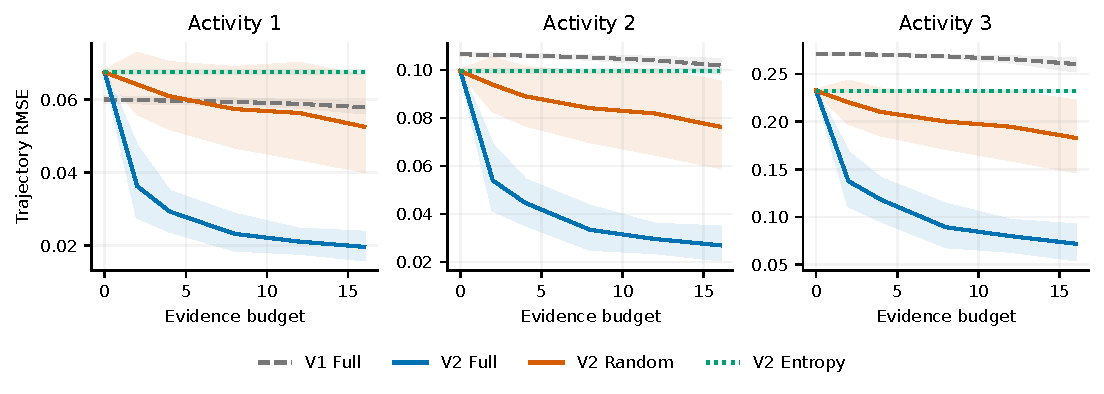
\includegraphics[width=\linewidth]{v2_budget_curves.pdf}
\caption{第二阶段冻结测试的逐活动曲线。阴影为逐点的 95\% 世界 bootstrap 区间。V2 的三种取证共用先验与更新；V1 使用原始校准。ParamIG 与 V2 Full 重合，为便于阅读省略。}
\label{fig:v2-curves}
\end{figure}
\begin{table}[tbp]
\centering\small
\setlength{\tabcolsep}{4pt}
\caption{逐活动的冻结测试结果。每个活动模板有 24 个独立世界实现；同一世界内的活动不视为独立。}\label{tab:v2-activities}
\begin{tabular}{llrll}
\toprule
版本 & 活动 & AUC & AUC 的 95\% 区间 & B0--B16 的 95\% 区间 \\
\midrule
V1 & 1 & 0.05911 & [0.05831, 0.05992] & [0.00109, 0.00358] \\
V1 & 2 & 0.10486 & [0.10382, 0.10567] & [0.00228, 0.00785] \\
V1 & 3 & 0.26770 & [0.26578, 0.26916] & [0.00519, 0.01849] \\
V2 & 1 & 0.02769 & [0.02393, 0.03177] & [0.04375, 0.05123] \\
V2 & 2 & 0.04041 & [0.03429, 0.04726] & [0.06506, 0.07858] \\
V2 & 3 & 0.10519 & [0.09004, 0.12190] & [0.14057, 0.17774] \\
\bottomrule
\end{tabular}
\end{table}


\paragraph{哪些变化有效，哪些结论仍不成立。}
30 组配置产生了 18 个不同的开发 AUC。在最终核宽下，将有效机制数下限从 8 提高到 24 没有改变权重，因为未触发温度提升时的有效机制数已超过 24。因此，护栏可以拒绝不合格候选，但最终配置的改善不能全部归因于护栏主动抬高温度。在核宽 .008、过程权重 8 不变时，将更新温度从 1 调到 .5，AUC 从 0.08193 降至 0.07569；温度 2 则恶化到 0.09056。这是可直接比较的温度实验。其他配置组同时改变核宽、过程权重或损失聚合方式，不能据此单独确定每个因素的因果贡献。移除批量幻想分支条件化后，匹配配置的选择记录和分数相同，这个证据池没有展示独立的批量去冗余收益。

证据池固定包含 24 条查看记录、40 条概率已知为 .5 的可用性记录，以及 96 条边缘化意图记录。最大熵策略将预算花在不可约的可用性随机性上，查看记录则能区分歧义的注意机制。这种设计使失效原因容易解释，也限定了结论：它有利于具有信息敏感性的选择策略，不能证明任意证据池上的普遍优势。测试增益大于开发增益，与固定历史条件下不同的取证答案有关，开发集仅含 12 个世界。当前证据支持“构造场景中恢复了主动取证价值”，尚不支持真实世界机制识别、新的未知规则告警保证或任何官方榜单成绩。

